\chapter{Human-Aware Probabilistic Planning}
\label{chapter:mamdp}

\lhead{Chapter 9. \emph{Human-Aware Probabilistic Planning}} % Change X to a consecutive number; this is for the header on each page - perhaps a shortened title

In this section we present a recent work where we developed a Multi-Agent Markov Decision Process (MAMDP). Section~\ref{sec:mamdp-intro} presents the problem. Section~\ref{sec:mamdp-overview} briefly introduces our approach, which is explained fully in section~\ref{sec:mamdp-single_agent} and section~\ref{sec:mamdp-mamdp}. Section~\ref{sec:mamdp-discussion} discusses the characteristics of this model, while section~\ref{sec:mamdp-example} show an example of creation of an MAMDP, starting from single-agent models. Finally, section~\ref{sec:mamdp-plan_monitoring} proposes an extension to the plan monitoring algorithm previously introduced, that would allow our system to monitor tasks and evaluate human engagement in collaborative activities.


\section{Introduction}
\label{sec:mamdp-intro}
Multi-Agent planning   is an important and studied topic in the AI community \citep{durfee1999survey}. There are several approaches to this problem, using classical or probabilistc planning. There are several issues to consider:
\begin{itemize}
\item Distributed vs Centralized. A multi-agent planner might be distributed, meaning that separate systems plan independently and then communicate to build a shared plan (an idea investigated, for example in \cite{nikolaidis2013cross,guestrin2002distributed} ); or centralized, meaning that a single system plans for all the agents.
\item Coordination. Agents need to coordinate their plans, in particular in the presence of shared resources. Imagine, for example, two agents, Max and Bob, that are using a tool to repair a set of cars. If Max is proceeding faster than Bob and the two do not coordinate, Max might take the tool and leave, starting to repair another car, ignoring the fact that Bob still needs the tool. This example shows that it is important to reason on the duration of actions performed by agents. At the simplest level, agents need to know the advancament of the sub-plan of other agents. More complex reasoning might take into account how long an agent needs to perform a certain sub-task, in order to refine a plan. 
\item Cooperation. Even when performing different sub-tasks of the same plan, agents can help each other, for example by passing items, thus improving the efficiency of the plan. Multi-Agent problems can be loosely or tightly coupled, depending on the quantity of interactions between agents. Some works are not focused specificly on tightly or loosely problems, and try to present a generic approach. \cite{torreno2015approach} proposes a cooperative refinement planning approach, based on the partial-order planning paradigm. In this work each agent refines a centralized plan. Agents are able to exchange information, since the complete world-state might not be observable by all of the agents. Refined plans are then analyzed by each agents, and voted with a democratic leadership approach. Results show that this approach is very efficient at solving loosely coupled problems, but also competent on tightly coupled situations. 

\item Communication and Knowledge. In a multi-agent environment each agent might have an incomplete or incorrent belief on the world, which might lead to wrong or sub-optimal actions. Agents may communicate to progressively build a correct belief model on the state world. 
\end{itemize}

Several approaches has been studied to bring the multi-agent planning problem in a probabilistic framework. \cite{boutilier1999sequential} create a centralized MDP, able to select at each time step actions for every present agent. Dec-POMDP \cite{bernstein2002complexity} and I-POMDP \cite{gmytrasiewicz2005framework} are more complex frameworks, that take into account the belief models of agents. The complexity of these models makes them difficult to use in even moderately difficult scenarios. A solution to this problem is considering simpler problems, where the agents mostly work independently and interact only in limited situations, such as in \cite{melo2013heuristic}.  Since we are more interested in tightly coupled scenarios, where the robot and human interact often, these kind of approaches are not suitable.

\section{Overview}
\label{sec:mamdp-overview}
In some situations, the environment, or other agents' actions, can be very unpredictable, and the system needs to constantly adapt its plans to the current state of the world, by replanning or repairing processes, which can be expensive. To deal with this issue we developed a Human-Aware Probabilistic Planner, based on MDPs. Our goal is replicating the characteristics of HATP, which we presented in section~\ref{sec:plan_management-hatp}, in a probabilistic domain. We designed this planner with the following ideas:

\begin{itemize}
\item Centralization. We will use a single planner, which chooses actions for all the involved agents.
\item Hierarchical. The domain will be split in different modules, which interact to solve the issue. Hierarchical models allow us to speed up the computation of the MDP policy and to reuse models in different domains and tasks.
\item Tightly Coupled. We will focus on problems where the agents' interactions are frequent.
\item No Communication. The planner will  assume that all the agents have perfect knowledge of the world state. The rest of the system will have to take care of maintaining users' knowledge, ensuring the correct execution of the plan. Current planners that try to include communication issues often focus on loosely coupled interactions between the agents, in order to simplify the domain and be able to compute a policy for the problem. Since we choose to focus on tightly coupled problems, we can not use this solution, and so prefer to avoid the issue at this level.
\end{itemize}

This work is a very recent development, and has not yet been integrated in the rest of the system. We will explain the main characteristics of the MAMDP in the following sections.


\section{Single-Agent MDP}
\label{sec:mamdp-single_agent}
The starting point for this planner is the single agent MDP. We start with the classical model $(S,A,T,C,G,S_0)$, where $S$ is the system space, $A$ is the set of actions, $T(s_i,a,s_j)$ is the probability to transition from state $s_i$ to state $s_j$ after taking action $a$, $C(s,a)$ is the cost of taking action $a$ in state $s$, $G \in S$ is the set of goal states, and $S_0 \in S$ is the set of starting states. We express the state space $S$ of the system as a set of variables $var$, each one with a possible range of values $values(v)$, where $v$ is a variable.

 We develop this model in the following way.

\subsection{Parameters}
We can define parameters in our MDP, and assign them to different values. We will call the list of parameters of an MDP $par$ and their current instantiation the \textit{parameter\_instance} of the model. Parameters can be linked to variables and values. We call $par\_var$ the variables associated to a parameter. 

For example, let us imagine a scenario of a room, with different furniture and objects. Let us define the state space of a generic MDP to take an object in this room. We can define two variables: the location of an agent, \textit{agent\_isAt}, which can assume values in the set ${f_1, f_2, f_3}$ (where $f_i$ represent a furniture in the room); and an object variable, \textit{object\_isAt}, which can assume the same values as the \textit{agent\_isAt} variable. If we define two parameter variables, \textit{agent} and \textit{object}, and link them to the \textit{agent\_isAt} and \textit{object\_isAt} variables, we can create a generic MDP which can be used to plan for any agent (with similar capacities) to take an object in this room.

The MDP receives as input, when consulted to select an action, the state of the world,  which we will call \textit{real\_space}. The \textit{real\_space} will be converted, using the \textit{parameter\_instance}, to the \textit{parameter\_space}, which will be actually used by the model in its computations. 

For example, in the real world, we have two agents, \textit{Bob} and \textit{Greg}, and three objects \textit{glue}, \textit{book}, \textit{smartphone}. If we assign the \textit{agent} parameter to \textit{Bob} and the \textit{object} parameter to \textit{book}, when receiving the complete world state the MDP will assign as \textit{agent\_isAt} the location of Bob, and as \textit{object\_isAt} the location of the book, discarding unneeded variables.

Parameters allow us to create smaller, generic MDPs, which can be reused easily.


\subsection{Actions and Macro Actions}
We define actions as a tuple $(subject,action\_name,object,target)$, where each element of the tuple is called an $action\_part$.  We represent the action as a string, composed by its $action\_parts$, joined by the character `\_' as delimiter. For example, an action where Greg places a book on a table can be represented as \textit{Greg\_place\_book\_table}. We define the function $convertPar(a)$ and $convertReal(a)$ to convert action $a$ to the \textit{real\_space} or the \textit{parametrized\_space}.

We add to the normal set of actions of an MDP \textit{macro actions}, linked to other MDPs, which allow us to create a hierarchy of MDPs. We call $M$ the set of \textit{macro actions} of the MDP, and $sub(a)$ the sub-MDP linked to the \textit{macro action} $a$. For example, we might create, in an MDP whose goal is cleaning a room, a macro action to reorder the room's object and one to clean the floor. Each of these macro actions will be linked to a specific MDP, who will refine the problem in more details.

The cost of executing a macro is directly computed from the sub-MAMDP. There are several strategies to compute this cost, like in \cite{dietterich2000hierarchical,hauskrecht1998hierarchical}.

\section{Name and Parameter Name}
We define for each MDP model a \textit{name}, which identifies it, and a \textit{parametrized\_name}, which substitutes parameters using the \textit{parameter\_instance}. The \textit{name} is defined using the same tuple as an action. 

For example, an MDP whose goal is to obtain an object could have as \textit{name} $agent\_get\_object$ and as \textit{parametrized\_name}, in a certain moment, $Greg\_get\_book$.

We define a function $assignParameterFromActionName(a)$ which creates the \textit{parameter\_instance} of the MDP based on an action name. This function can be very useful when using \textit{macro actions}, so that the system can assign parameters to the sub-MDP from the \textit{macro action} string and then consult it.

For example, if the \textit{macro action} $Greg\_get\_book$ is linked to the $agent\_get\_object$ MDP, this function would assign values to the  $agent\_get\_object$ model's parameter. The system would assign the value $Greg$ to the $agent$ parameter and the value $book$ to the $object$ parameter. 

Each \textit{name} can be divided in a number of $name\_parts$,  with the same procedure as actions. The \textit{parametrized\_name} can be divided as well in $parametrized\_parts$.


\subsection{Abstract States}

In some situations, a model might not need to base its planning choices on all the possible values of a variable in the \textit{real\_space}. Imagine, for example, the case where an agent needs to perform a series of operations on the furniture $f_1$ in the room. In this case, we could model the  values of the \textit{agent\_isAt} variable as $\{f_1 , other\_location\}$, greatly reducing the state space. In this situation we say that \textit{agent\_isAt} is an \textit{abstract variable}. 

We build a map $abstract\_values_v$ for each abstract variable $v$, which links real world values to model values (e.g. $f_2 \rightarrow other\_location$). This map will be used to convert a state expressed in the $real\_space$ to the $parameter\_space$ of the model. 
%The choice of using abstract variables needs to be carefully weighted, because they can impact on the quality of the solution of the model.

\section{Multi-Agent MDP}
\label{sec:mamdp-mamdp}
Now we will explain how we build a Multi-Agent MDP (MAMDP), starting from $n$ single-agent models, one for each agent. We will call the single-agent models $MDP_i$, where $1 \leq i \leq n $ is the index of the agent. In the following paragraphs, we will use the notion $S_i, var_i, values_i, A_i, T_i, C_i, G_i, S_{0i}, M_i, par_i, par\_var_i$ when referring to components of the single-agent MDP, adding the $i$ index to differentiate them from the MAMDP. 
 
\subsection{Name and Parameter Name}
The \textit{name} and \textit{parameter\_name} of the MAMDP are built by concatenating those of its agent MDPs, adding the `-' character to separate the single agents.

For example, the \textit{name} of a MAMDP with single-agent models \textit{agent\_get\_object} and  \textit{agent\_clean\_table} is \textit{agent\_get\_object-agent\_clean\_table}.

\subsection{State Space and Parameters}
$par=\bigcup_{1 \leq i \leq n, p \in par_i} p+\text{`p'}+i $. \\
$par\_var=\bigcup_{1 \leq i \leq n, v \in par\_var_i} \> rename(v)$ \\
$var=\bigcup_{i=1}^{n}(var_i \setminus par\_var_i) \cup par\_var$ \\
$\forall_{v \in var}\> value(v)=\bigcup_{i| v \in var_i} 
\begin{cases}
	 value_i(v) \quad \text{if } v \not \in par_i \\
	 p+\text{`p'}+i \quad \text{if } v \in par_i \\
\end{cases}$ \\ 

To create the set of parameters of the MAMDP we will rename each parameter in the single-agent MDPs, adding an identifier composed by `p' and by the index of the MDP. We make this choice because different MDPs could share the same parameters, but they could be assigned to different values, and so need to be treated as separate entities, even if they have the same semantic meaning. Parameter variables are created by renaming the parameter variables of the sub-MDPs to account for this newly added identifier.

For example, if the $MDP_1$ model has a parameter \textit{object}, linked to a variable called \textit{object\_isAt}, we will rename the parameter as \textit{objectp1} and the variable as \textit{objectp1\_isAt}. 

We defined $S$ as the union of the variables of the single-agent MDPs excluding their parameter variables. We will instead take the parameter variables of the MAMDP, in the way that we just defined.

The MAMDP variable can assume all the possible values that are available in the corresponding variables of the sub-MDPs. As before, we will change values that are parameters to account for our renaming procedure. 

We define the function $single_i(s)$ , which converts the MAMDP state to state of the single-agent MDP $i$.


\subsection{Actions}
$A=(\prod_{i=1}^{n} A_i) \cup JointActions \cup WaitActions$ , where $JointActions$ is the set of collaborative actions, and $WaitActions$ is a set computed by enumerating all the possibile instances where one or more agents do not act, and simply wait, while others are acting.

The actions of the MAMDP are a concatenation of the actions of the single MDP, adding the separator character `-' between the different agents' actions. We will refer to the single agent's actions of action $a$ as $a_i \quad \forall \> 1\leq i \leq n$.

For example, the MAMDP will contain actions such as `agentp1\_move\_surface1-agentp2\_move\_surface2'.

We add to $A$ the special set of $JointActions$, which are actions that the agents can use to cooperate. For example, if there is a resource in a single agent MDP which two agents can possess, we introduce a $handover$ action between them. 

For each $a \in A$, if there is a sub-action $a_i$ which is a macro action for MDP $i$, we create a new MAMDP and assign it as sub-MAMDP of $a$. This sub-MAMDP will be created from $n$ MDP models, as for its father, in the following way. Let $f$ be the father MAMDP, $c$ the sub-MAMDP, and $a$ the macro-action of $f$. \\
 $ \forall_{\text{MDP}\> m_i \in f}$ we assign an MDP $m_j$ in $c$ where:\\
$m_j= \begin{cases}
	m_i & \quad \text{if } a_i \not\in M_i \\
	sub_i(a_i) & \quad \text{if } a_i \in M_i 
\end{cases}$ \\

\subsection{Transition Function}
$T(s_a,a,s_b)=
\begin{cases}
\prod_{i=1}^{n}(T_i(single_i(s_a),a_i,single_i(s_b))) & \> \text{if } !isIncongruent(s_a)\; \land  \;!isIncongruent(s_b)  \\
0   & \quad \text{else}
	\end{cases}$ \\

The transition function is computed as the product of the transition functions of the single agent MDPs, on the converted states and actions.

We set the probability as zero if either the starting or ending states state of the transition are incongruent. This is done by converting the states to the \textit{real\_space} and checking the values of the different variables. We say that a state is incongruent if two non abstract variables in the \textit{parameter\_space}, that are assigned to the same \textit{real\_space} variable, have different values. If one or both the variables are abstract we check if their $abstract\_values$, for the current variable values, have a value in common. If not, we consider the state incongruent.

For example, consider the state $(objectp0\_isAt=`surface', objectp1\_isAt=`table', agentp0\_isAt=`table', agentp1\_isAt=`table')$. If in the current \textit{parameter\_instance} both \textit{objectp0} and \textit{objectp1} are assigned to the same variable, this state will be incongruent.

Consider now the state $(objectp0\_isAt=`agentp0', objectp1\_isAt=`other', agentp0\_isAt=`table', \\ agentp1\_isAt=`table')$. If $agentp0$ is a parameter assigned to $Greg$, \textit{objectp1\_isAt} is an abstract variable, and $abstract\_values_{objectp1\_isAt}(`Greg')=`other'$, this state will not be considered incongruent.  

\subsection{Cost Function}
$C(s_a,a,s_b)= 
	\begin{cases}
		max_{i=1}^{n}(C_i(single_i(s_a),a_i,single_i(s_b))  & \quad \text{if } s_b \not\in G \\
		\sum_{i | single_i(s_a) \in G_i} expectedCost_i(single_i(s_a))  & \quad \text{if } s_b \in  G
		\\
	\end{cases} $	\\

where $expectedCost_i(s)$ is a function that computes the expected cost for agent $i$ to reach a goal state by starting in state $s$ and following the action policy. In this calculation, we allow from the other agent only $JointActions$ that are necessary to solve the plan (e.g. handovers if the agent does not have a needed resource).

The cost function of the MAMDP is chosen by taking the maximum cost of the single agent actions that are executed, if the state $s_b$ is not a goal state. If it is a goal state, we take as cost an estimation of the time required by the other agents to complete their tasks, with only minimal cooperation. In this way, we encourage the MAMDP to choose plan where the agents cooperate and do not only try to achieve their goal.

\subsection{Start and Goal States}
$S_0=\bigcap_{i=1}^n S_{0i}$. The starting states of the MAMDP is set to the intersection of the single agents starting states.\\\\$G=\bigcup_{i=1}^n G_i $, where $G_i$ is the set of goal states of a single agent MDP. The goal states of the MAMDP is the intersection of the single agent goal states. The idea of this choice is that an MAMDP terminates when one of the agents has achieved its goal. If there is an agent that has not completed its task, and the MAMDP was a sub-model in a hierarchy, its father will select another action, perhaps assigning one or more agents to the incompleted task. 

In some situations, we might try creating a MAMDP composed of opposing goals, like for example, an MAMDP where both agents need to get the same object. Since we are interested in cooperative and not competitive scenarios, we will not create this MAMDPs. We can recognize them since $G$ will be empty, as the single-agent goal sets do not have states in common.

\section{Discussion}
\label{sec:mamdp-discussion}

The result of this fusion is an MDP, that can be solved with well-known algorithms, like value iteration. By fusing all the possible MDPs, the resulting model can be  very hard to solve but, using macro actions, parameters, and abstract states we can greatly reduce its complexity. 

The action space of the joint model is calculated as the cross product of the action spaces of the single model. When there are several macro actions in the agent models, this could result in the creation and computation of the policy of several sub-models, which can significantly slow down the computation of a solution for the model. We can reduce this process by making several considerations.

First of all, created MAMDPs can be reused in different branches of the hierarchy, if needed. When creating a new MAMDP, we will look to see if there is already an existing MAMDP with the same $name$ and, if so, we will use it.

Second, parameters can greatly  reduce the number of sub-MAMDPs to compute. Let $a$ be a \textit{macro action}, $c$ the sub-MAMDP linked to $a$, $1..n$ the indexs of the single-agent MDPs of $c$, which are selected as previously explained.

 We create the \textit{parametrized\_name} of $c$ by concatenating the \textit{parametrized\_name} of its single-agent MDPs. To set the $name$ of  $c$ we process each name of its single-agent MDPs $name_i$, by modifying all of its $name\_parts_{i,k}$, with $1 \leq k \leq m$ in the following way:\\
$name\_part_{i,k}=
\begin{cases}
	name\_part_{i,k} & \quad \text{if } !parametersInCommon(name\_part_{i,k}) \\
	parametrized\_part_{i,k} & \quad \text{else}
\end{cases}$ \\
where $parametersInCommon(name\_part_{i,k})$ is a function that returns true if $name\_part_{i,k}$ is a parameter in sub-MDP $i$, and there is a sub-MDP with index $j$, where $name\_part_{i,k}$ is a parameter or variable. \\

The idea behind this choice is the following. If the sub-MDPs do not have parameters in common, we can use a generic MAMDP to represent this instance. For example, if we create an MAMDP for the macro action $agent1\_clean\_table-agent2\_clean\_shelf$, we can use the MAMDP $agent\_clean\_furniture-agent\_clean\_furniture$ since the sub-MDP models do not have parameters in common, and their actions will not conflict.

 If instead we create an MAMDP for the macro action $agent1\_clean\_table-agent2\_clean\_table$ we create a specialized MAMDP, since there are parameters in common ($table$) and if we treat them as different objects there could be incongruences in the MAMDP planning.



\section{Example}
\label{sec:mamdp-example}
In this section we will show an example of creation of a MAMDP. We start by presenting a cooperative scenario. The robot and a human are working together to assemble three brackets on three differents work surfaces. To assemble a bracket the agents need to clean the surface, apply some glue to it, and fix the bracket. A possible set-up for this scenario is shown in figure ~\ref{fig:mamdp-mamdp_scenario}.

 \begin{figure}[ht!]
	\centering
	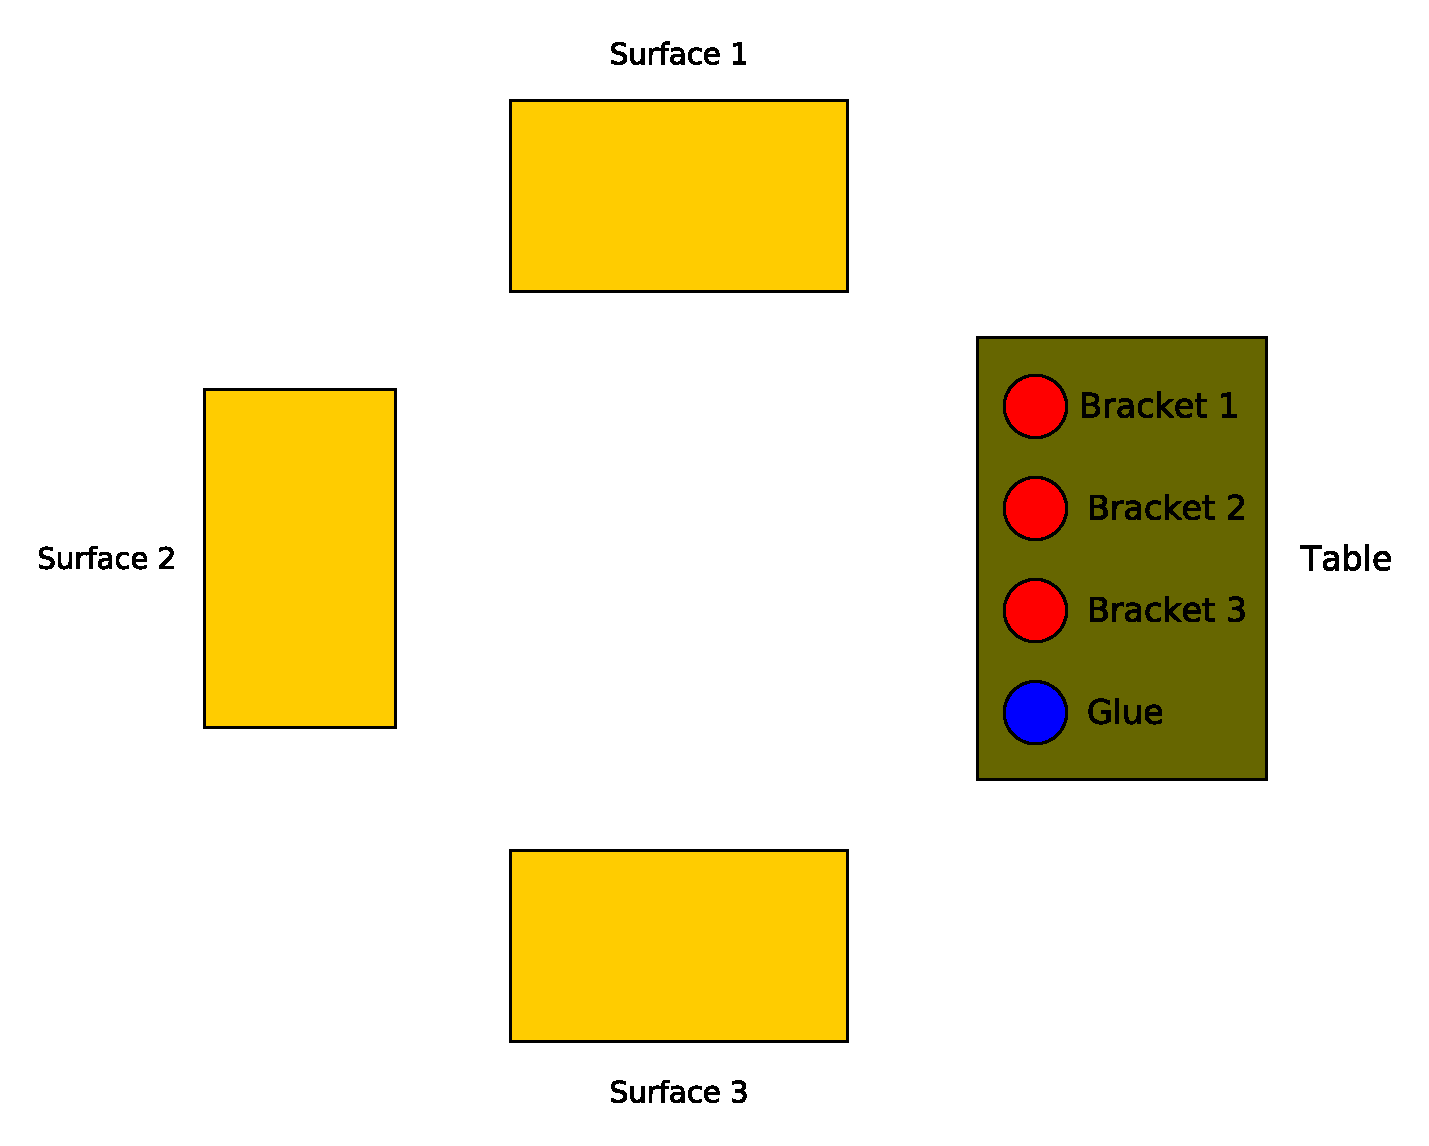
\includegraphics[scale=0.5]{img/coworker/mamdp/scenario.pdf}
	\caption[MAMDP example scenario]{The image shows the set-up for this example scenario. The four locations are represented as different rectangles and the objects as circles. }
	\label{fig:mamdp-mamdp_scenario}
\end{figure}

\subsection{Single-Agent MDP}

We start by defining a single-agent MDP for this scenario. We will use a hierarchical architecture, as shown in figure~\ref{fig:mamdp-scenario_single_architecture}. This architecture is composed by three different modules: AssembleAllBrackets, which controls the flow of the scenario; AssembleBracketSurface, which assembles a chosen bracket on a chosen surface; and GetObject, which obtains an object. We will create some simplifications in these models, as they are chosen just to explain how we build a MAMDP, and not for a realistic use.

\begin{figure}[ht!]
	\centering
	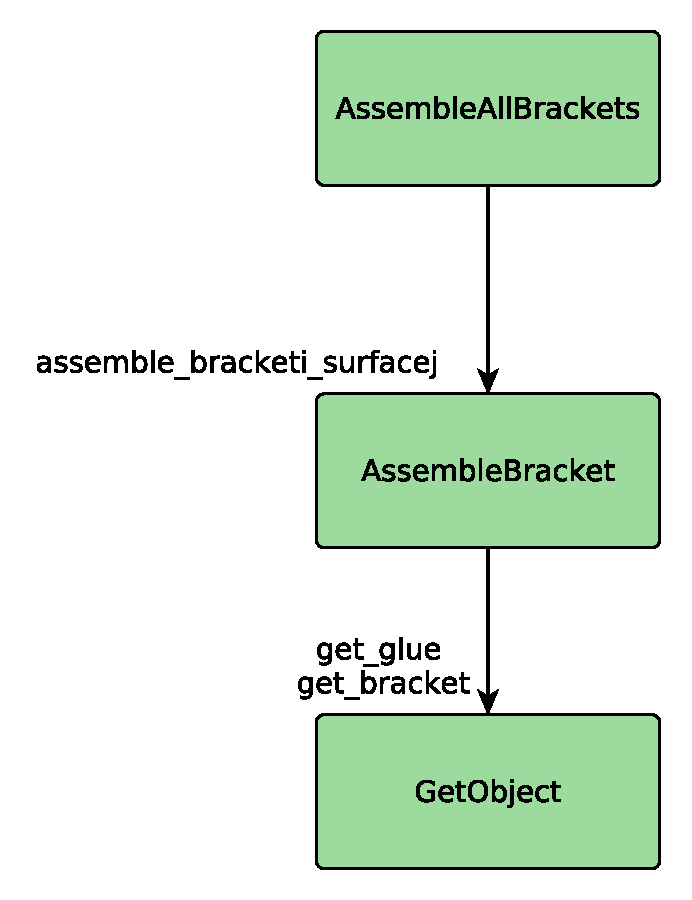
\includegraphics[scale=0.5]{img/coworker/mamdp/scenario_single_architecture.pdf}
	\caption[MAMDP example single MDP]{The image shows the architecture for the single agent MDP of the MAMDP example scenario. The various MDPs are represented as rectangles. The arrows show the links between hierarchical modules in the architecture. The label of the arrow shows the macro action corresponding to the link. The label \textit{assemble\_bracketi\_surfacej} actually correspond to all the combinations to assemble a bracket on a surface. We grouped them since, as the AssembleBracketSurface MDP uses parameters, it can be used for all these macros.}
	\label{fig:mamdp-scenario_single_architecture}
\end{figure}



\subsubsection{AssembleAllBrackets}
We will now show the \textit{AssembleAllBrackets} model, whose goal is directing the flow of the scenario, by choosing which bracket should be assembled on which surface.

\begin{itemize}
	\item $name: agent\_assembleallbrackets$.
	\item		$par: agent$
		\begin{itemize}
			\item $par\_var(agent)=agent\_isAt$
		\end{itemize}
		In this example, we decided to create generic models which can plan either for Greg or for the robot.
	\item $S:\;\{agent\_isAt,bracket1\_isAt,bracket2\_isAt,bracket3\_isAt,surface1\_status,\\ surface2\_status,surface3\_status\}$. 
		\begin{itemize}
			\item $values(agent\_isAt):\{table,surface1,surface2,surface3\}$.
			\item $values(bracketi\_isAt):\{table,surface1,surface2,surface3,agent,other\_agent\} \forall_{i=1}^3$. 
			\item $values(surfacei\_status):\{completed,other\_status\}\;\forall_{i=1}^3$.
		\end{itemize}
		\begin{itemize}
			\item $abstract\_values\_surfacei\_status:$ 
				\begin{itemize}
					\item $none: other\_status$.
					\item $cleaned: other\_status$.
					\item $glued: other\_status$.
				\end{itemize}
			\item $abstract\_values\_bracketi\_isAt$ 
				\begin{itemize}
					\item $greg: other\_agent$.
					\item $robot: other\_agent$.
				\end{itemize}	
		\end{itemize}
		The state set of the model contains the location of the agent, of the brackets, and the status of the surfaces. The agent and the objects can be located at the table or at one of the surfaces. In addition, objects can be possessed by another agent. The status of a surface can be set to none, meaning that the fixing process as not started; cleaned, meaning that the agent has already cleaned the surface; glued, meaning that the agent has applied glue to the surface; and completed, meaning the a bracket ha been fixed on it. 

		To simplify the model we consider the states $none,cleaned,glued$ as abstract states. We also consider $other\_agent$ as an abstract value, assigned to both agents present in the scenario. Let us consider, for example, that the instance of the \textit{agent} parameter is \textit{greg}, and that in the \textit{real\_space} \textit{bracket1\_isAt=greg}. It could seem that, when converting from \textit{real\_space} to \textit{parameter\_space} the system would assign \textit{bracket1\_isAt} to \textit{other\_agent}, since \textit{other\_agent} is an abstract value for \textit{greg}. In reality, the system will give priority to the current parameter, and execute the conversion properly, by setting \textit{bracket1\_isAt=agent}. 
	\item $A:\;\{agent\_assemble\_bracketi\_surfacej\}\;\forall_{i=1}^1 \forall_{j=1}^3$.
	\item $M: A$.

	All of this model's actions are actually \textit{macros}.
	\item $G:\; \cup_{s:S}\; |\; \forall_{i=1}^3\; surfacei\_status=completed\;\text{AND}\;\\
	forall_{i=1}^3\;\exists_{j}\;|\;bracketi\_isAt=surfacej\; \text{AND} \\
	\forall_{i,j=1}^3\; bracketi\_isAt \neq bracketj\_isAt.$

	The goal of this model is to fix all the brackets on the surfaces. We set as goal states every state in which the brackets are located on different surfaces and the status of each surface is \textit{completed}. 
	\item $S_0:\; \cup_{s:S}\;|\; \exists{1\leq i \leq 3}\; |\; surfacei\_status \neq completed$.

\end{itemize}

Note that we did not need to specify a cost function for this model. Since all of its actions are \textit{macros}, the cost function will be directly derived by its sub-models.

\subsubsection{AssembleBracket}
We will now show the \textit{AssembleBracket} model, whose goal is assembling a specific bracket on a specifc surface.
\begin{itemize}
	\item $name: agent\_assemble\_bracket\_surface$.
	\item		$par: \{agent,bracket,surface\}$
		\begin{itemize}
			\item $par\_var(agent)=agent\_isAt$
			\item $par\_var(bracket)=bracket\_isAt$
			\item $par\_var(surface)=surface\_status$
		\end{itemize}

	\item $S:\;\{agent\_isAt,bracket\_isAt,surface\_status,glue\_isAt\}$. 
		\begin{itemize}
			\item $values(agent\_isAt):\{surface,other\_location\}$.
			\item $values(bracket\_isAt):\{agent,surface, other\_location,other\_agent\}$. 
			\item $values(glue\_isAt):\{agent,other\_location,other\_agent\}$. 
			\item $values(surface\_status):\{none,cleaned,glued,completed\}$.
		\end{itemize}
		\begin{itemize}
			\item $abstract\_values\_bracket\_isAt$ 
				\begin{itemize}
					\item $surfacei=other\_location\; \forall_{i=1}^n$ .
					\item $table=other\_location$.
					\item $greg=other\_agent$.
					\item $robot=other\_agent$.
				\end{itemize}	
			\item $abstract\_values\_glue\_isAt=abstract\_value\_bracket\_isAt$ 
			\item $abstract\_values\_agent\_isAt$
				\begin{itemize}
					\item $surfacei=other\_location\; \forall_{i=1}^n$ .
					\item $table=other\_location$.
				\end{itemize}
		\end{itemize}
		
		This state set will contain, other than the variables of \textit{AssembleAllBrackets}, also the location of the glue bottle. In this situation, \textit{surface\_status} will not be an abstract variable, since the model needs to know what is the exact state of the fixing process. We greatly simplified the number of locations where agents and objects can be present by using abstract variables. This model is only interested in knowing if the agent has an object (glue or bracket) or not. In the case where the agent does not have an object, it can invoke the \textit{get\_object macro}, which will take charge of obtaining it, using a more complete state space.
	\item $A:\;\{agent\_move\_surface,agent\_clean\_surface,agent\_glue\_surface,\\
	agent\_fix\_bracket,agent\_get\_bracket,agent\_get\_glue\}$.
	\item $M:\;\{agent\_get\_bracket,agent\_get\_glue\}$.
	\item $G:\; \cup_{s:S}\; |\; surfacei\_status=completed$
	\item $S_0:\; \cup_{s:S}\; |\; surfacei\_status \neq completed$
\end{itemize}


\subsubsection{GetObject}
We will now show the \textit{GetObject} model, whose goal is obtaining an object in the environment.

\begin{itemize}
	\item $name: agent\_get\_object$.
	\item		$par: \{agent,object\}$
		\begin{itemize}
			\item $par\_var(agent)=agent\_isAt$
			\item $par\_var(object)=object\_isAt$
		\end{itemize}

	\item $S:\;\{agent\_isAt,object\_isAt\}$. 
		\begin{itemize}
			\item $values(agent\_isAt):\{table,surface1,surface2,surface3\}$.
			\item $values(object\_isAt):\{table,surface1,surface2,surface3,agent,other\_agent\}$. 
		\end{itemize}
		\begin{itemize}
			\item $abstract\_values\_object\_isAt$ 
				\begin{itemize}
					\item $greg=other\_agent$.
					\item $robot=other\_agent$.
				\end{itemize}	
		\end{itemize}
		The state set of this model contains a more detailed representation of the possible locations of the scenario, since the goal of the agent is obtaining an object.		

	\item $A:\;\{agent\_move\_table, agent\_move\_surface1\, agent\_move\_surface2, \\ 
	agent\_move\_surface3, agent\_take\_object\}$.
	\item $M:\;{\emptyset}$.
	\item $G:\; \cup_{s:S} \; | \; object\_isAt=agent$
	\item $S_0:\; \cup_{s:S} \; | \; object\_isAt \neq agent$
\end{itemize}

\subsection{MAMDP}
We will now show how our MAMDP is created. The MAMDP hierarchy, shown in figure~\ref{fig:mamdp-scenario_mamdp_architecture} will contain different models. At the highest level lies the model \textit{AssembleAllBracket-AssembleAllBracket}, a duplication for two agents of the highest top module. The lowest modules include different combinations of the single agent sub-MDPs, in order to account for the possible task assignations. We will start by showing the top MAMDP model.

\begin{sidewaysfigure}[ht!]
	\centering
	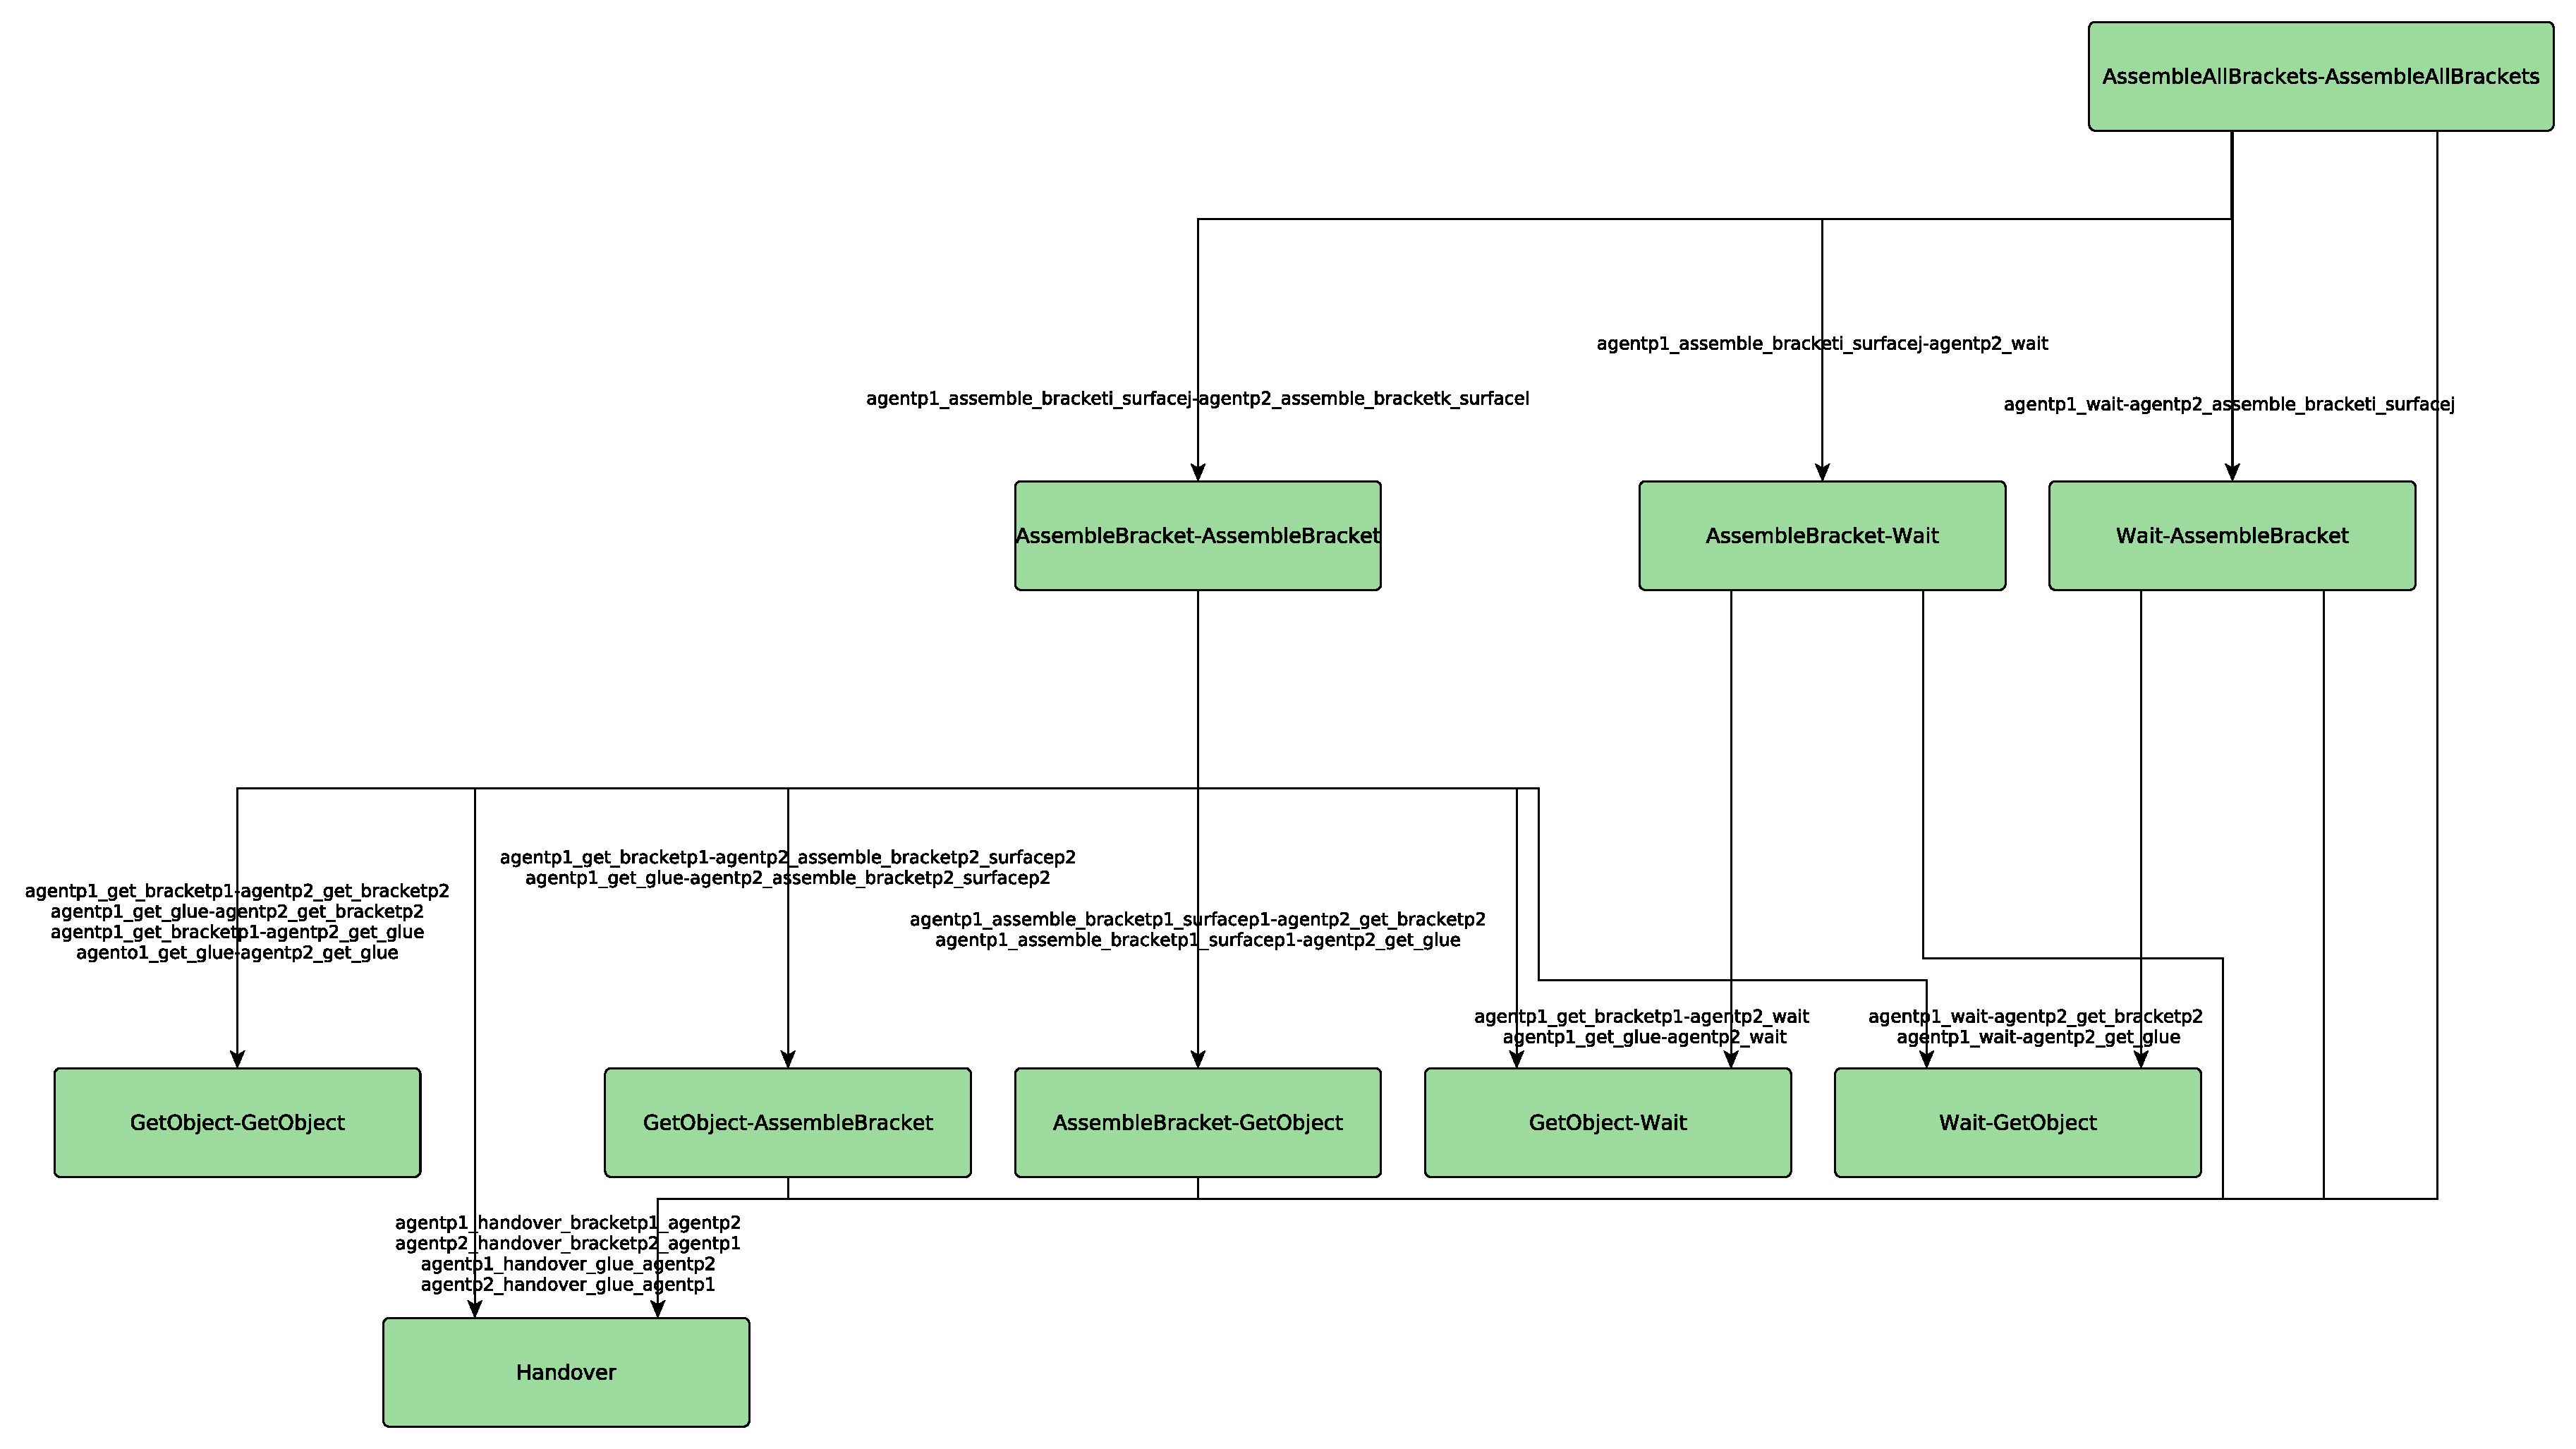
\includegraphics[scale=0.4]{img/coworker/mamdp/scenario_mamdp_architecture.pdf}
	\caption[MAMDP example single MDP]{The image shows the architecture for the MAMDP for the example scenario. The various MAMDPs are represented as rectangles. The arrows show the links between hierarchical modules in the architecture. The label of the arrow shows the macro action corresponding to the link.}
	\label{fig:mamdp-scenario_mamdp_architecture}
\end{sidewaysfigure}


\subsubsection{AssembleAllBrackets-AssembleAllBrackets}
\begin{itemize}
	\item $name: agent\_assembleallbrackets-agent\_assembleallbrackets$.
	\item		$par: \{agentp1,agentp2\}$.
		\begin{itemize}
			\item $par\_var(agentp1)=agentp1\_isAt$.
			\item $par\_var(agentp2)=agentp2\_isAt$.
		\end{itemize}

		The name of the parameters are changed, adding \textit{pi} at the end, where \textit{i} is the index of the agent. This allows to assign them in an unique way.
	\item $S:\;\{agentp1\_isAt,agentp2\_isAt, bracket1_isAt,bracket2_isAt,bracket3_isAt,\\
	surface1\_status,surface2\_status,surface3\_status\}$. 
		\begin{itemize}
			\item $values(agentp1\_isAt):\{table,surface1,surface2,surface3\}$.
			\item $values(agentp2\_isAt):\{table,surface1,surface2,surface3\}$.
			\item $values(bracketi\_isAt):\{table,surface1,surface2,surface3,agentp1,agentp2\}\; \forall_{i=1}^3$. 
			\item $values(surfacei\_status):\{completed,other\_status\}\;\forall_{i=1}^3$.
		\end{itemize}
		\begin{itemize}
			\item $abstract\_values\_surfacei\_status:$ 
				\begin{itemize}
					\item $none: other\_status$.
					\item $cleaned: other\_status$.
					\item $glued: other\_status$.
				\end{itemize}
		\end{itemize}
		The state set is not very different, simply accounting for the presence of two agents.

	\item $A:\;\{agentp1\_assemble\_bracketi\_surfacej-agentp2\_assemble\_bracketk\_bracketl\}\;\forall_{i=1}^1 \forall_{j=1}^3
	\forall_{k=1}^3 \forall_{l=1}^3 \cup JointActions \cup WaitActions$.
	\item $JointActions=agentpi\_handover\_bracketj\_agentpl \; \forall_{i=1}^2 \; \forall{j=1}^3 \; \forall_{l=1; l!=i}^3$.
	\item $WaitActions=(agentp1\_assemble\_bracketi\_surfacej-agentp2\_wait \; \cup \\
	 agentp1\_wait-agentp2\_assemble\_bracketi\_surfacej) \; \forall_{i=1}^3 \; \forall_{j=1}^3$.

	The action set is the cartesian product of the actions of the single models, plus actions to exchange brackets, plus actions where only one agent is acting.
	\item $M: A$.
	\item $G:\; \cup_{s:S}\; |\; \forall_{i=1}^3\; surfacei\_status=completed\;\text{AND}\\
	\forall_{i=1}^3\; \exists_{j}\;|\;bracketi\_isAt=surfacej\; \text{AND}\\
	\forall_{i=1}^3\; bracketi\_isAt \neq bracketj\_isAt$.
	\item $S_0:\; \cup_{s:S} \; \exists{1\leq i \leq 3}\; |\; surfacei\_status \neq completed$.

	The starting and goal states are the same as the single-agent model. Since the two models used to create the MAMDP are the same, the intersection and union of the states will be the same
\end{itemize}


If we would create and solve a new MAMDP for each of these macro, we would create a great quantity of models. Fortunately, as previously said, we can reduce this number by creating generic sub-models for a macro that can be used when there are not parameters in common. In this case, we actually need to create a single sub-MDP for every action of the type \textit{agentp1\_assemble\_bracketi\_surfacej-agentp2\_assemble\_bracketk\_surfacel}, where $i=j$ or $j=l$ (since they would have variables in common), plus a generic sub-MAMDP for all the other cases. Actually, in this case, these specific MDPs would not be created, since they are considered not valid, as the intersection of their goal states is null (since a bracket can not be on two surfaces at the same time and a surface can not contain more than one bracket).


\subsubsection{AssembleBracket-GetObject}
Let us consider the AssembleBracket-GetObject MDP, deeper in the hierarchy. In this case, we will need to create a generic sub-MAMDP, plus specific MDPs for the macros \textit{agentp1\_assemble\_bracketi\_surfacej-agentp2\_get\_bracketi} and \textit{agentp1\_assemble\_bracketi\_surfacej-agentp2\_get\_glue}, since they share resources. We will show parts of this sub-MAMDP.  


\begin{itemize}
	\item $name: agent\_assemblebracket-agent\_getobject$.
	\item		$par: \{agentp1,bracketp1,surfacep2,agentp2,objectp2\}$.
		\begin{itemize}
			\item $par\_var(agentp1)=agentp1\_isAt$.
			\item $par\_var(bracket1)=bracketp1\_isAt$.
			\item $par\_var(surfacep1)=surfacep1\_status$.
			\item $par\_var(agentp2)=agentp2\_isAt$.
			\item $par\_var(object2)=objectp2\_isAt$.
		\end{itemize}

	\item $S:\;\{agentp1\_isAt, bracketp1\_isAt,surfacep1\_status, glue\_isAt, agentp2\_isAt, objectp2\_isAt\}$. 
		\begin{itemize}
			\item $values(agentp1\_isAt):\{surfacep1,other\_location\}$.
			\item $values(bracketp1\_isAt):\{agentp1,surface, other\_location,other\_agent\}$. 
			\item $values(glue\_isAt):\{agentp1,other\_location,other\_agent\}$. 
			\item $values(surfacep1\_status):\{none,cleaned,glued,completed\}$.
			\item $values(agentp2\_isAt):\{table,surface1,surface2,surface3\}$.
			\item $values(objectp2\_isAt):\{table,surface1,surface2,surface3,agentp2,other\_agent\}$. 
		\end{itemize}
		\begin{itemize}
			\item $abstract\_values\_objectp2\_isAt:$ 
				\begin{itemize}
					\item $greg=other\_agent$.
					\item $robot=other\_agent$.
				\end{itemize}	
			\item $abstract\_values\_bracketp1\_isAt:$ 
				\begin{itemize}
					\item $surfacei=other\_location \forall_{i=1}^n$ .
					\item $table=other\_location$.
					\item $greg=other\_agent$.
					\item $robot=other\_agent$.
				\end{itemize}	
			\item $abstract\_values\_glue\_isAt=abstract\_value\_bracketp1\_isAt$ 
			\item $abstract\_values\_agentp1\_isAt:$
				\begin{itemize}
					\item $surfacei=other\_location \forall_{i=1}^n$ .
					\item $table=other\_location$.
				\end{itemize}
		\end{itemize}

	\item $G:\; \cup_{s:S}\; |\; surfacep1\_status=completed\; \text{OR} \; objectp2\_isAt=agentp2$
	\item $S_0:\; \cup_{s:S} \; | \; surfacep1\_status=completed \; \text{AND} \; objectp2\_isAt \neq agentp2$

	The goal and starting states of the model are, respectively, the union and intersection of the single models.
\end{itemize}


\subsubsection{Handover}
Finally, to conclude, we show the special handover MAMDP, used for cooperative actions. Since this is a special model, not created by joining two single-agent MDPs, it will not follow the same rules, and instead it will be treated in a similar way as a single agent MDP.

\begin{itemize}
	\item $name: agent1\_handover\_object\_agent2-agent2\_receive\_object\_agent2$.
	\item		$par: \{agent1,object,agent2\}$
		\begin{itemize}
			\item $par\_var(agent1)=agent1\_isAt$
			\item $par\_var(agent2)=agent2\_isAt$
			\item $par\_var(object)=object\_isAt$
		\end{itemize}

	\item $S:\;\{agent1\_isAt, agent2\_isAt, object\_isAt\}$. 
		\begin{itemize}
			\item $values(agent1\_isAt):\{surface1,surface2,surface3,table\}$.
			\item $values(object\_isAt):\{agent1,agent2,other\_location\}$. 
			\item $values(agent2\_isAt):\{surface1,surface2,surface3,table\}$. 
		\end{itemize}
		\begin{itemize}
			\item $abstract\_values\_object2\_isAt:$ 
				\begin{itemize}
					\item $table=other\_location$.
					\item $surface1=other\_location$.
					\item $surface2=other\_location$.
					\item $surface3=other\_location$.
				\end{itemize}	
		\end{itemize}

	\item $A:\;\{agent1\_move\_location-agent2\_move\_location, agent1\_move\_location-agent2\_wait,\\agent1\_wait-agent2\_move\_location, \\ 
	agent1\_give\_object\_agent2-agent2\_receive\_object\_agent1\} \\ \text{where}\; location \in \{table,surface1,surface2,surface3\}$
	\item $G:\; \cup_{s:S} \; | \; object\_isAt=agent2$
	\item $S_0:\; \cup_{s:S} \; | \; object\_isAt=agent1$
\end{itemize}



\section{Enhancing Task Monitoring}
\label{sec:mamdp-plan_monitoring}

In section~\ref{sec:plan_management-plan_monitoring} we introduced the problem of task monitoring. We presented three different problematics: monitoring actions, monitoring tasks, and evaluating human engagement.

We presented a solution only for the problem of monitoring actions. In this section, we propose a strategy to monitor tasks and evaluate the human's engagement, based on the MAMDP model developed in this chapter. We are just starting to investigate this idea, and have not yet completed an implementation.

In general, a MAMDP proposes only the next action in the plan, which is not sufficient to manage plans and ensure synchronism. To deal with this problem, we can compute an horizon of $h$ actions from the MAMDP, building causal links between the nodes to create the stream structure introduced in chapter~\ref{chapter:plan_management}.

\subsection{Evaluating Human Engagement and Monitoring Tasks}
Understanding if a human is engaged in a task is equivalent to infer if its current intention is to achieve the task. As previously said, in section~\ref{subsec:intention-unknown_intentions}, normally, this module is not able to monitor joint goals. To solve this issue, while performing a shared plan, we create, in the Situation Assessment layer, a new intention for each MAMDP model in the domain. We associate to these intentions the linked MAMDP and the context node \textit{have a shared plan}, which is treated as evidence with a true value. We call these intentions \textit{plan intentions}.

We associate to each known intention a precomputed \textit{expected length}, which is the expected time to accomplish the linked goal.

Using the Intention and Action Recognition module, the robot can infer which is currently the most likely human intention. If the current intention equals the task to monitor, the robot infers that the human is actively working to complete its task.

 We consider the task, and the monitor procedure, as \textit{completed} when the linked MAMDP reaches a \textit{goal state}.

If the human is currently not involved in the monitored task there are three possibilities:
\begin{itemize}
	\item The human has momentarily interrupted the task. This can be inferred if the human is currently involved in another intention, which does not belong to the \textit{plan intentions}, and whose expected length is \textit{short}. In this case, the monitor procedure will not return an error until a predefined \textit{allowed time}.
	\item The human has abandoned the task.  This can be inferred if the human is currently involved in another intention, which does not belong to the \textit{plan intentions}, and whose expected length is \textit{long}. The monitor will return a \textit{not involved error}. 
	\item The human is performing another task in the shared goal. This can be inferred if the human is currently involved in another intention, which belongs to the \textit{plan intentions}. In this case the monitor will return an \textit{other task error}. 
\end{itemize}




